\documentclass{clbeamer2024}

\usepackage{minted}

\usepackage{minted}
\setminted{
	breaklines=true,
	frame=single,
	bgcolor=lightgray,
	fontsize=\small,
	escapeinside=||
}

\usepackage{xcolor}
\definecolor{bg}{rgb}{0.95, 0.95, 0.92} % Couleur gris clair

\title{
	%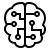
\includegraphics[width=0.5cm]{logos/IA1.png} \hfill
        Introduction à la Blockchain
	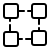
\includegraphics[width=0.55cm]{logos/Blockchain.png} \hfill
}
\subtitle{Comprendre les bases de la blockchain et ses applications}
\author{Slimani Mohamed Amine}
\institute{EHTP}
\date{\today}

\begin{document}
	\setcounter{framenumber}{-1}
	\frame{\titlepage}
	
	
	
	% Sommaire
	\begin{frame}{Sommaire}
		\tableofcontents
	\end{frame}
	
	\section{Qu'est-ce que la Blockchain ?}
	\begin{frame}{Qu'est-ce que la Blockchain ?}
		\begin{itemize}
			\item \textbf{Définition} : Une blockchain est un registre distribué et décentralisé qui enregistre les transactions de manière sécurisée et transparente.
			\item \textbf{Caractéristiques} :
			\begin{itemize}
				\item \textbf{Décentralisation} : Pas de contrôle centralisé.
				\item \textbf{Transparence} : Toutes les transactions sont visibles par tous les participants.
				\item \textbf{Immuabilité} : Les données ne peuvent pas être modifiées après leur enregistrement.
			\end{itemize}
		\end{itemize}
	\end{frame}


\section{Composants de la Blockchain}
\begin{frame}{Composants de la Blockchain}
	\begin{itemize}
		\item \textbf{Blocs} : Contiennent des transactions et sont liés entre eux.
		\item \textbf{Noeuds} : Les participants du réseau qui valident et enregistrent les transactions.
		\item \textbf{Mining} : Processus de validation des transactions et de création de nouveaux blocs.
	\end{itemize}
\end{frame}

\section{Types de Blockchains}
\begin{frame}{Types de Blockchains}
	\begin{itemize}
		\item \textbf{Blockchain publique} : Accessible à tous (ex : Bitcoin, Ethereum).
		\item \textbf{Blockchain privée} : Contrôlée par une organisation spécifique.
		\item \textbf{Blockchain hybride} : Combinaison de blockchain publique et privée.
	\end{itemize}
\end{frame}


\section{Applications de la Blockchain}
\begin{frame}{Applications de la Blockchain}
	\begin{itemize}
		\item \textbf{Cryptomonnaies} : Bitcoin, Ethereum.
		\item \textbf{Contrats intelligents} : Exécution automatique de contrats.
		\item \textbf{Supply Chain} : Traçabilité des produits.
		\item \textbf{Vote électronique} : Sécurité et transparence des votes.
	\end{itemize}
\end{frame}


\section{Exemple de transaction sur la Blockchain}
\begin{frame}{Exemple de transaction sur la Blockchain}
	\begin{enumerate}
		\item Un utilisateur initie une transaction.
		\item La transaction est diffusée sur le réseau.
		\item Les noeuds valident la transaction.
		\item La transaction est ajoutée à un bloc et enregistrée sur la blockchain.
	\end{enumerate}
\end{frame}


\section{Bonnes pratiques}
\begin{frame}{Bonnes pratiques}
	\begin{itemize}
		\item \textbf{Sécurité} : Utiliser des clés privées sécurisées.
		\item \textbf{Scalabilité} : Choisir des blockchains adaptées à vos besoins.
		\item \textbf{Conformité} : Respecter les régulations locales.
	\end{itemize}
\end{frame}

\section{Outils pour travailler avec la Blockchain}
\begin{frame}{Outils pour travailler avec la Blockchain}
	\begin{itemize}
		\item \textbf{Ethereum} : Plateforme pour les contrats intelligents.
		\item \textbf{Hyperledger} : Framework pour les blockchains d'entreprise.
		\item \textbf{Truffle} : Environnement de développement pour Ethereum.
	\end{itemize}
\end{frame}


\section{Pourquoi c'est important ?}
\begin{frame}{Pourquoi c'est important ?}
	\begin{itemize}
		\item La blockchain est une technologie clé pour la décentralisation, la transparence, et la sécurité des transactions.
		\item Elle est utilisée dans des domaines tels que la finance, la supply chain, et les contrats intelligents.
		\item Comprendre la blockchain est essentiel pour les développeurs et les professionnels de la technologie.
	\end{itemize}
\end{frame}


\begin{frame}{Résumé}
	\textbf{La blockchain} est une technologie révolutionnaire pour la décentralisation, la transparence, et la sécurité des transactions.  
	Explorez, apprenez, et innovez avec la blockchain !
\end{frame}
	

	
	
\end{document}
